\subsection{Theory of MoC}
The key assumptions are the flow is inviscid and irrotational. For such flows the complete velocity governing equation can be written as:\\
\begin{center}
    $ (1 - \frac{u^2}{a^2})\frac{\partial u}{\partial x} + (1 - \frac{v^2}{a^2})\frac{\partial v } {\partial y } - \frac{2uv}{a^2}\frac{\partial du}{\partial dy} = 0$
\end{center}\\
The velocity of any supersonic flow can be broken down such that one of its two components has speed of sound, from the above equation when $u$ equals $a$, $\frac{\partial u}{\partial x}$ becomes indeterminate, and it remains indeterminate along the line $\sin{\mu} = \frac{a}{V}$. Such lines are called characteristic lines, which are also the mach waves. It can be shown that
\begin{center}
    $ (\frac{dy}{dx})_{char} = \tan(\theta \mp \mu) $\\
    $  \theta + \nu(M) = K$_-$  $\\
    $  \theta - \nu(M) = K$_+$  $\\
\end{center}
\begin{figure}[H]
    \centering
    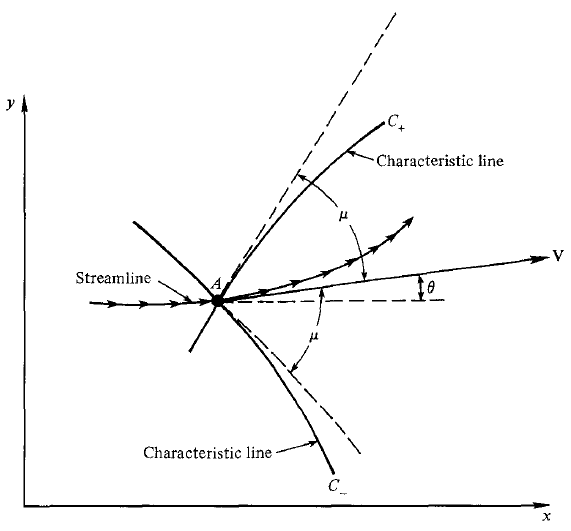
\includegraphics[width=0.5\textwidth]{text/Characteristic lines.PNG}
    \caption[Characteristic line]{Slope of characteristic line (Source [1])}
    \label{fig:Slope of characteristic line}
\end{figure}
When two characteristics are intersecting at a point, then the flow angle $\theta$ and prandlt meyer function $\nu$ can be estimated using\\
\begin{center}
    $  \theta_1 + \nu(M)_1 = K$_-$_1 = K$_-$_3 = \theta_3 + \nu(M)_3 $\\ 
    $  \theta_2 - \nu(M)_2 = K$+-$_1 = K$+-$_3 = \theta_3 - \nu(M)_3 $\\ 
    \end{center}
\begin{figure}[H]
    \centering
    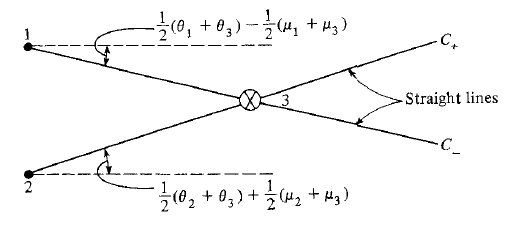
\includegraphics[width=0.5\textwidth]{text/intersection_characterisitcs.PNG}
    \caption[Intersection of Characteristics]{Intersection of Characteristics (Source [1])}
    \label{fig:Intersection of Characteristics}
\end{figure}    
Assuming the slope angle of mach lines is the average of the slope angles, the coordinates of the third point can be calculated from\\
\begin{center}
    $\frac{y_3 - y_2}{x_3 - x_2} = \tan(0.5(\theta_3 + \theta_2) + 0.5(\nu_3 + \nu_2) )  $\\
    $\frac{y_3 - y_1}{x_3 - x_1} = \tan(0.5(\theta_3 + \theta_1) - 0.5(\nu_3 + \nu_1) )  $\\
\end{center}
\subsection{Nozzle Design}
Key assumptions
\begin{enumerate}
\setlength\itemsep{0.01em}
    \vspace{-2mm}
    \item Inviscid and Irrotational
    \vspace{-2mm}
    \item Characteristics are only slightly curved
\end{enumerate}
The diverging section of the nozzle generally consists of expansion section and straightening section. The slope of the nozzle contour at the expansion fan is continuously increasing, or in other words the function of the nozzle contour at the expansion section is monotonously increasing hence it generates expansion waves and as well as reflects the incident expansion waves. The slope of the nozzle contour at the straightening section is monotonously decreasing, hence it terminates all the expansion waves incident on it. So the junction of expansion and straightening section has the highest slope($\theta_{max}$) in the nozzle wall contour. For a minimum length nozzle there is only a straightening section, as expansion section would just add on to excess mass. Henceforth the word nozzle is used instead of minimum length nozzle. At the throat there is a discontinuity in the slope of the nozzle contour. At this junction expansion fan emanates, which consists of series of expansion waves. At point 'A'\\
\\
   \theta$_{exp}$ = \nu(M$_2$) - \nu(M$_1$)\\
    \theta$_{max}$ = \nu$_A$ | Since 'A' is a sonic point, $\nu(M = 1) = 0$, hence K$_+$ = 0\\
    \theta$_{max}$ + \nu$_A$ = (K$_-)_A$\\ 
    (K$_-)_A$ = \theta$_{exit}$ + \nu$_{exit}$ as both the points lie on the same characteristic\\
    \theta$_{exit}$ = 0 | Imposing the condition that the flow has to emerge parallel to the center at the exit
    line\\
    \theta$_{max}$ = \nu$_A$ = \nu$_{exit}$/2\\
\\
\begin{figure}[H]
    \centering
    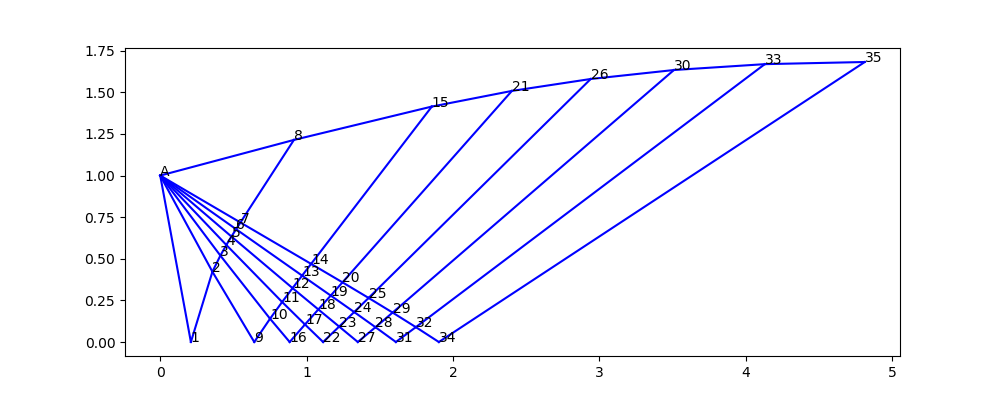
\includegraphics[width=1\textwidth]{text/MoC_Mine_Blue.png}
    \caption{Minimum Length Nozzle}
    \label{fig:Minimum Length Nozzle}
\end{figure}
So to design a nozzle, the first requirement is the exit mach number. And the slope at the throat corner point is decided by the prandlt meyer function at the exit point. All the points on the centerline has $\theta$ as zero, hence the mach number at the last point lying on the centerline has the same mach number as the design exit mach number. For the supersonic nozzle design, the algorithm to find the nozzle contour is as follows:
\begin{enumerate}
\setlength\itemsep{0.01em}
    \item Design the exit mach number and evaluate $\theta_{max}$
    \item Decide the number of characteristics required, say N
    \item At point 1, we assume$\dag$ $\theta_1$ a finite non-zero value, say 0.01$^0$, since K_+ = 0, \theta$_1$ = \nu$_1$ for all the points 1, 2... N, N+1
    \item We assume$\dag$  that for points 2,3...N flow angle $\theta$ is $\Delta\theta$ = $\theta_{max}/(N-1)$ inclined with $\theta_1$
    \item Assume the first set of characteristics are straight lines
    \item There are two approaches to find the slope:
    \begin{enumerate}
        \item Assuming the angle between the characteristics is also $\Delta\theta$
        \begin{enumerate}
            \item $\frac{x_i - x_a}{y_a - y_i} = \tan(\theta_i+\theta_1)$ for all i $\in {2...N}$    
        \end{enumerate}
        \item Assuming the slope angle of the line has contribution only from the points 1,2...N
        \begin{enumerate}
            \item $\frac{y_i - y_a}{x_i - x_a} = \tan(\theta_i - \nu_i )$ for all i $\in {1,2...N} $
        \end{enumerate}
    \end{enumerate}
    \item For contour points $0.5(\theta_a + \theta_i)$ is the slope angle
\end{enumerate}\\

\begin{figure}[H]
    \centering
    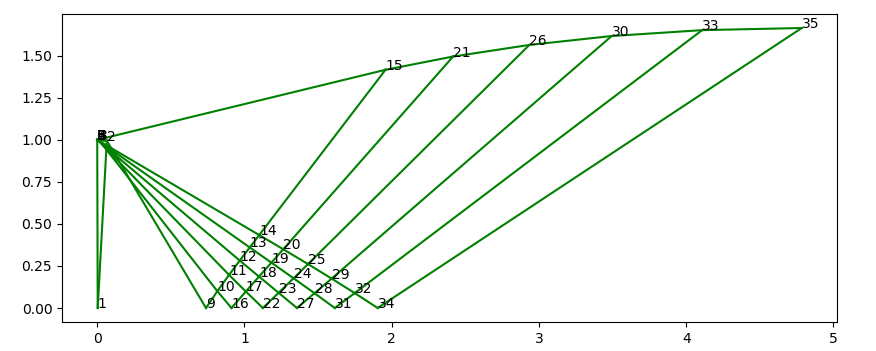
\includegraphics[width=0.8\textwidth]{text/MoC_Anderson.PNG}
    \caption[MOC Method I]{MOC Method I}
    \label{fig:MOC Method I}
\end{figure}

\begin{figure}[H]
    \centering
    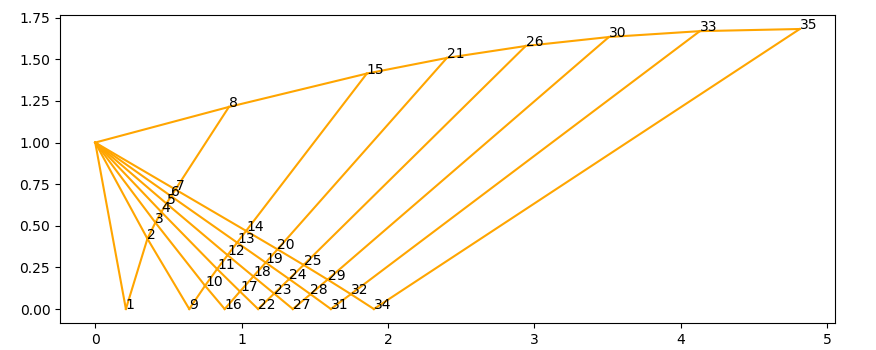
\includegraphics[width=0.8\textwidth]{text/MoC_Mine.png}
    \caption[MOC Method II]{MOC Method II}
    \label{fig:MOC Method I}
\end{figure}\\
\newpage
\begin{flushleft}
\textbf{Convergence}\\
\end{flushleft}
The values of Area ratio and length of the Nozzle converges when Number of Characteristics is about 30. But the variation is small even at lower number of characteristics. \\
\begin{center}
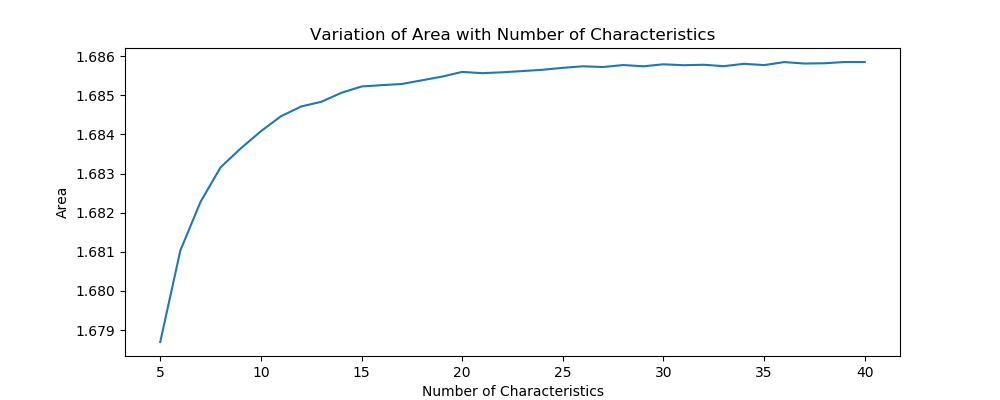
\includegraphics[width=0.8\textwidth]{text/Area Variation.png}\\
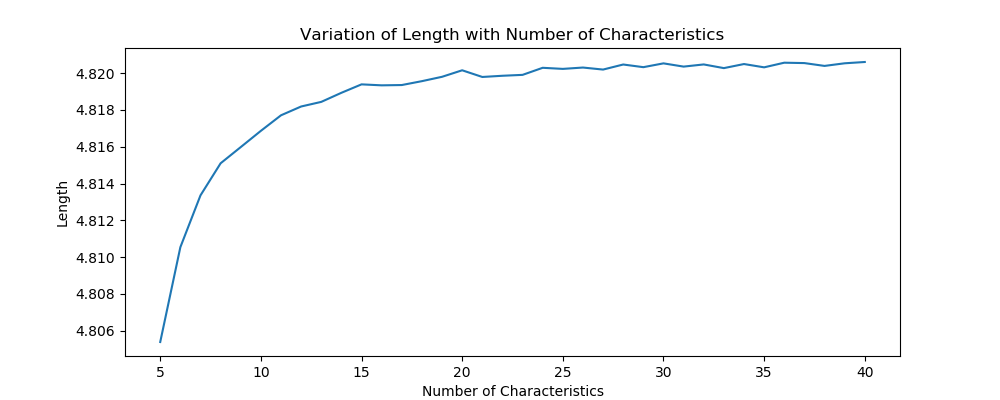
\includegraphics[width=0.8\textwidth]{text/Length Variation.png}\\    
\end{center}


\newpage
%\subsection{Nozzel Simulation using Time-Marching MacCormack Techinque}